\setcounter{secnumdepth}{4}
\lstdefinestyle{csharp}{
    language=C#,
    basicstyle=\ttfamily\small,
    commentstyle=\color{green!40!black},
    keywordstyle=\color{blue},
    numberstyle=\tiny\color{gray},
    numbers=left,
    stepnumber=1,
    numbersep=5pt,
    backgroundcolor=\color{white},
    showspaces=false,
    showstringspaces=false,
    showtabs=false,
    tabsize=2,
    frame=single,
    rulecolor=\color{black},
    captionpos=b,
    breaklines=true,
    breakatwhitespace=false,
    title=\lstname,
    escapeinside={\%*}{*)},
morekeywords={var},
}

\chapter{Produktspezifikationen}
Dieses Kapitel behandelt die Planung und Spezifikation des Projekts.
Weiteres wird die verwendete Technologieauswahl begründet und mit Alternativlösungen verglichen.

\section{Anforderungen und Spezifikationen}
Hier steht der allgemeine Text für die Anforderungen und Spezifikationen

\subsection{Use Cases}
Hier steht der allgemeine Text für die Use Cases

\section{Design}
Hier steht der allgemeine Text für das Design

\subsection{Abläufe}
Hier steht der allgemeine Text für die Abläufe

\subsection{Mockups}
Hier steht der allgemeine Text für die Mockups

\section{Eingesetzte Technologien}

\subsection{Kriterien}
Bei der Auswahl der eingesetzten Technologien war es besonders wichtig, dass diese möglichst
zuverlässig und bereits etabliert sind. Die Technologien sollen ausfallsicher, leicht benutzbar
und vorallem eine performant Verwendung der Applikation sicherstellen.

\subsection{Game Engine}
Als Game Engine wird eine Entwicklungsumgebung für das Design und Entwickeln von Spielen bezeichnet.
Zu Projektstart gab es die Auswahl zwischen den zwei bekanntesten Game Enginges, die momentan am Markt
vorhanden sind. Diese sind die folgenden:
\begin{itemize}
    \item Unreal Engine
    \item Unity
\end{itemize}

Nach tiefgründiger Recherche war für das Projektteam klar, dass Unity die verwendete GameEngine sein wird.
Folgende Kriterien haben uns in dieser Entscheidung verstärkt:
\begin{itemize}
    \item Programmiersprache: C#.
    \item Einfacher Einstieg in die Entwicklung von Spielen für Beginner.
    \item Sehr gute Dokumentation.
    \item Hohe Anzahl an Tutorials an die man sich richten kann.
\end{itemize}

% Hier dann beschreibeen wieso wir von Unreal Engine auf Unity umgestiegen sind.

\subsection{Unity foundation packages}
%Quellen:
In dem folgenden Abscnhitt wird erklärt welche Packages in die Unity Applikation
eingeführt werden müssen um die Entwicklung einer Augmented Reality Applikation ohne Problem
ermöglichen zu können.

\subsubsection{MRTK3}
Das Mixed Reality Toolkit (MRTK) \footnote{Microsoft \cite{MRTK3}} ist eine Sammlung von Tools,
Skripten und Ressourcen, die speziell für die Entwicklung von Mixed-Reality-Anwendungen, einschließlich Augmented
Reality, in Unity entwickelt wurden. MRTK3 ist eine Weiterentwicklung der vorherigen Versionen und bietet viele
Vorteile für AR-Anwendungen:
\begin{itemize}
    \item Interaktions- und Benutzerführung: \\
    MRTK3 stellt eine Reihe von Interaktionskomponenten und -systemen zur
    Verfügung, die es Entwicklern ermöglichen, intuitivere Benutzererfahrungen in AR-Anwendungen zu gestalten.
    Dies umfasst Dinge wie das Platzieren von Objekten in der realen Welt, die Verfolgung von Handgesten und die
    Unterstützung von Blickverfolgung.
    \item Standardisierte APIs: \\
    Durch die Verwendung von MRTK3 kannst du auf standardisierte APIs und Komponenten
    zugreifen, die speziell für AR-Anwendungen entwickelt wurden. Dies erleichtert die Implementierung von Funktionen
    wie Handgesten, Sprachsteuerung und Objektplatzierung.
    \item Einfache Konfiguration und Anpassung: \\
    MRTK3 bietet eine einfache Konfiguration und Anpassung über die
    Unity-Oberfläche. Dies erleichtert die Anpassung deiner AR-Anwendung an spezifische Anforderungen und Use Cases.
\end{itemize}

\subsubsection{Microsoft OpenXR Plugin}
Das Microsoft OpenXR Plugin \footnote{Khronos \cite{OpenXR}} ist eine Sammlung von Tools ist ein wichtiges Plugin für Unity, das die Integration von OpenXR-Unterstützung in
die AR-Anwendung ermöglicht. OpenXR ist ein offener Industriestandard, der die Entwicklung von XR
(Extended Reality)-Anwendungen, einschließlich Augmented Reality, erleichtert. Anschließend ein paar Punkte wieso
dieses Plugin so wichtig ist:
\begin{itemize}
    \item Geräteunabhängigkeit: \\
    Durch die Verwendung von OpenXR und dem Microsoft OpenXR Plugin kann die AR-Anwendung auf verschiedenen
    XR-Geräten ausgeführt werden, ohne die Kernfunktionalität für jedes einzelne Gerät neu entwickeln zu müssen.
    Dies gewährleistet eine reibungslose Interaktion mit der HoloLens 2 und anderen XR-Geräten.
    \item Leistungssteigerung und Stabilität: \\
    Die Nutzung von OpenXR und des Microsoft OpenXR Plugins kann die
    Leistung und Stabilität der AR-Anwendung erheblich verbessern. Sie gewährleisten eine reibungslose Ausführung
    der Anwendung auf dem Zielsystem und bieten eine optimale Benutzererfahrung.
\end[itemize]

\subsection{Modellierungsprogramm}

Die Erstellung der 3D-Modelle für die beiden Level erfordert ein Rendering-Programm. Die Entscheidung für das
Rendering-Programm Blender wurde bereits zu Beginn des Projekts getroffen. \\
Diese Wahl basiert auf folgenden Gründen:
\begin{itemize}
    \item \textbf{Kostenfrei und Open Source}\\
    Blender ist kostenfrei und quelloffen, was bedeutet, dass es ohne Lizenzkosten genutzt werden kann. Dies ist
    besonders attraktiv bei der Entwicklung von AR-Anwendungen mit begrenztem Budget.
    \item \textbf{Echtzeit-Rendering}\\
    Blender verfügt über einen Echtzeit-Renderer namens Eevee, der schnelle Vorschauen
    und Renderings ermöglicht. Dies ist hilfreich, um AR-Inhalte in Echtzeit anzuzeigen und zu überprüfen.

    \item \textbf{Integration mit AR-Frameworks}\\
    Obwohl Blender keine direkte Unterstützung für AR-Funktionen bietet, können die erstellten 3D-Modelle und
    Animationen in AR-Entwicklungsumgebungen wie Unity oder Unreal Engine importiert werden, um dort
    AR-spezifische Funktionalitäten hinzuzufügen.

\begin{comment}
% ALIBI BILDER KP WOHIN DAMIT UND SIND NICHT BESCHRIEBEN
\end{itemize}
\subsubsection{UI - Default ObjectMode}
\begin{figure}[h]
    \centering
    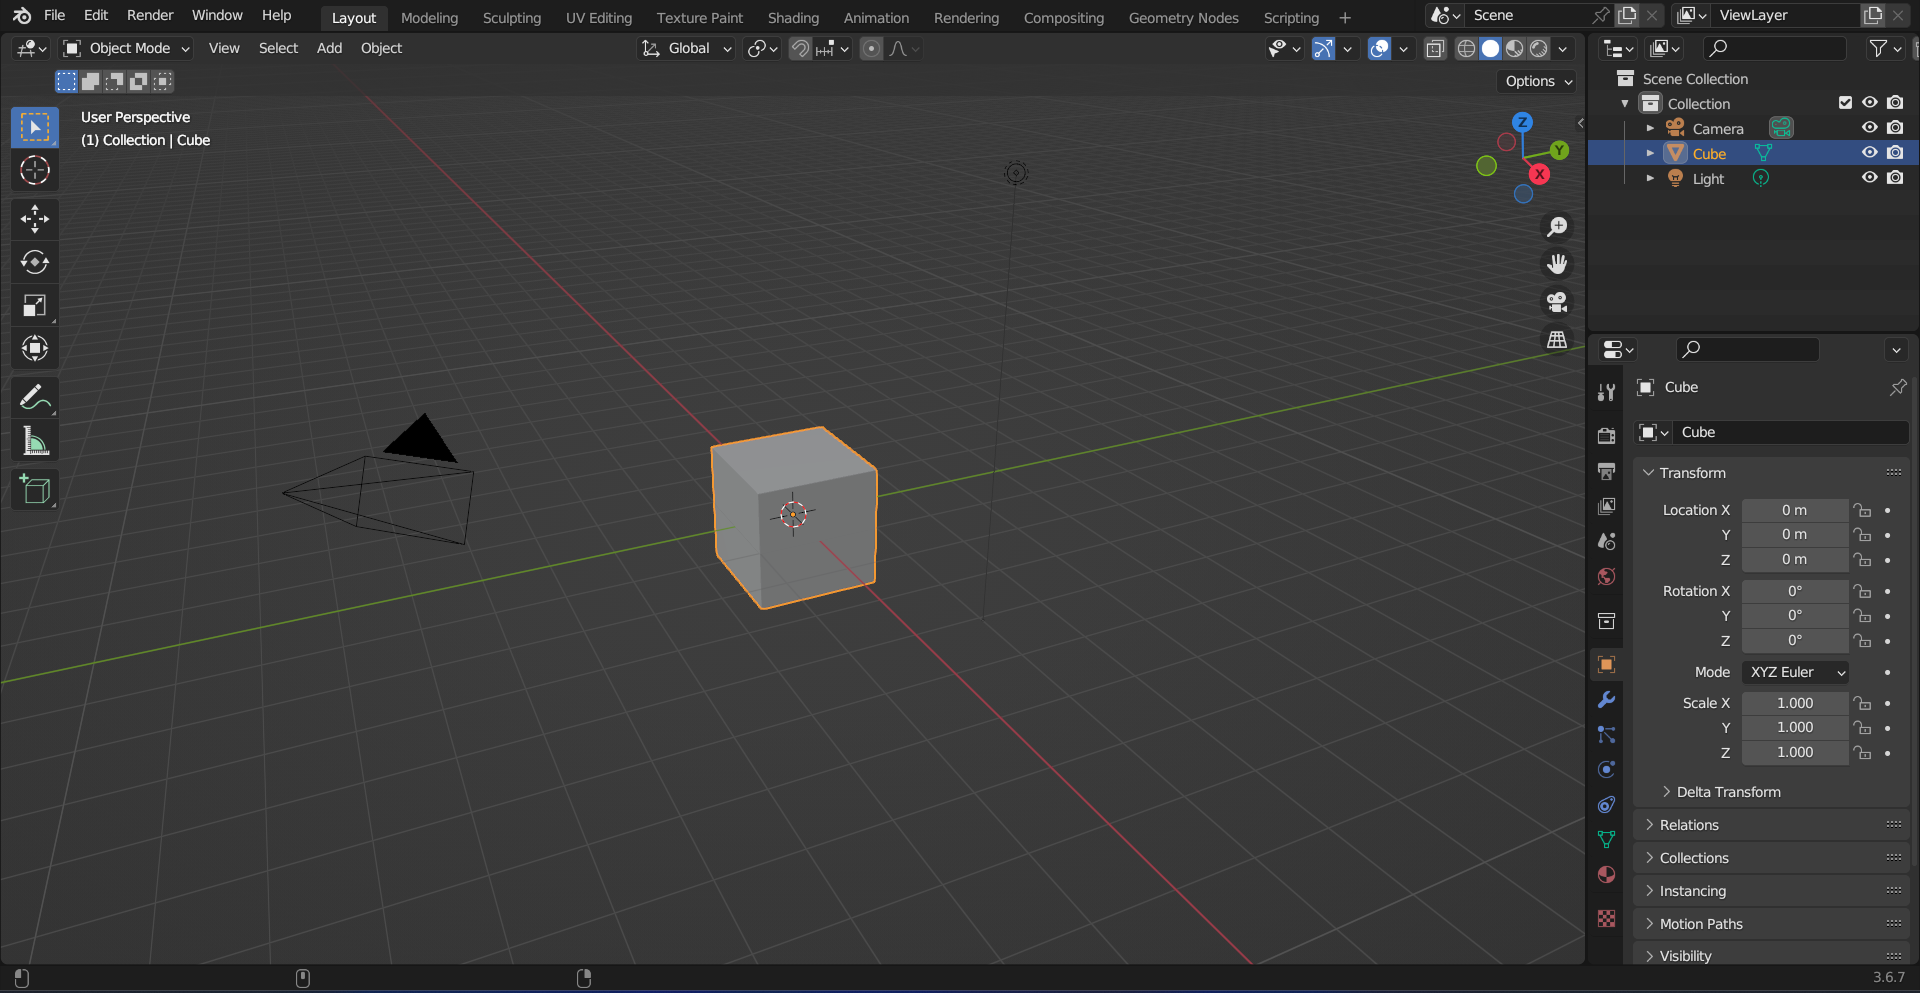
\includegraphics[width=1\textwidth]{images/defaultobjectmode.png}
    \caption{Standard File Ansicht im Object Mode}
    \label{fig:defaultobjectmode}
\end{figure}

\subsubsection{UI - Calculator EditMode}
\begin{figure}[h]
    \centering
    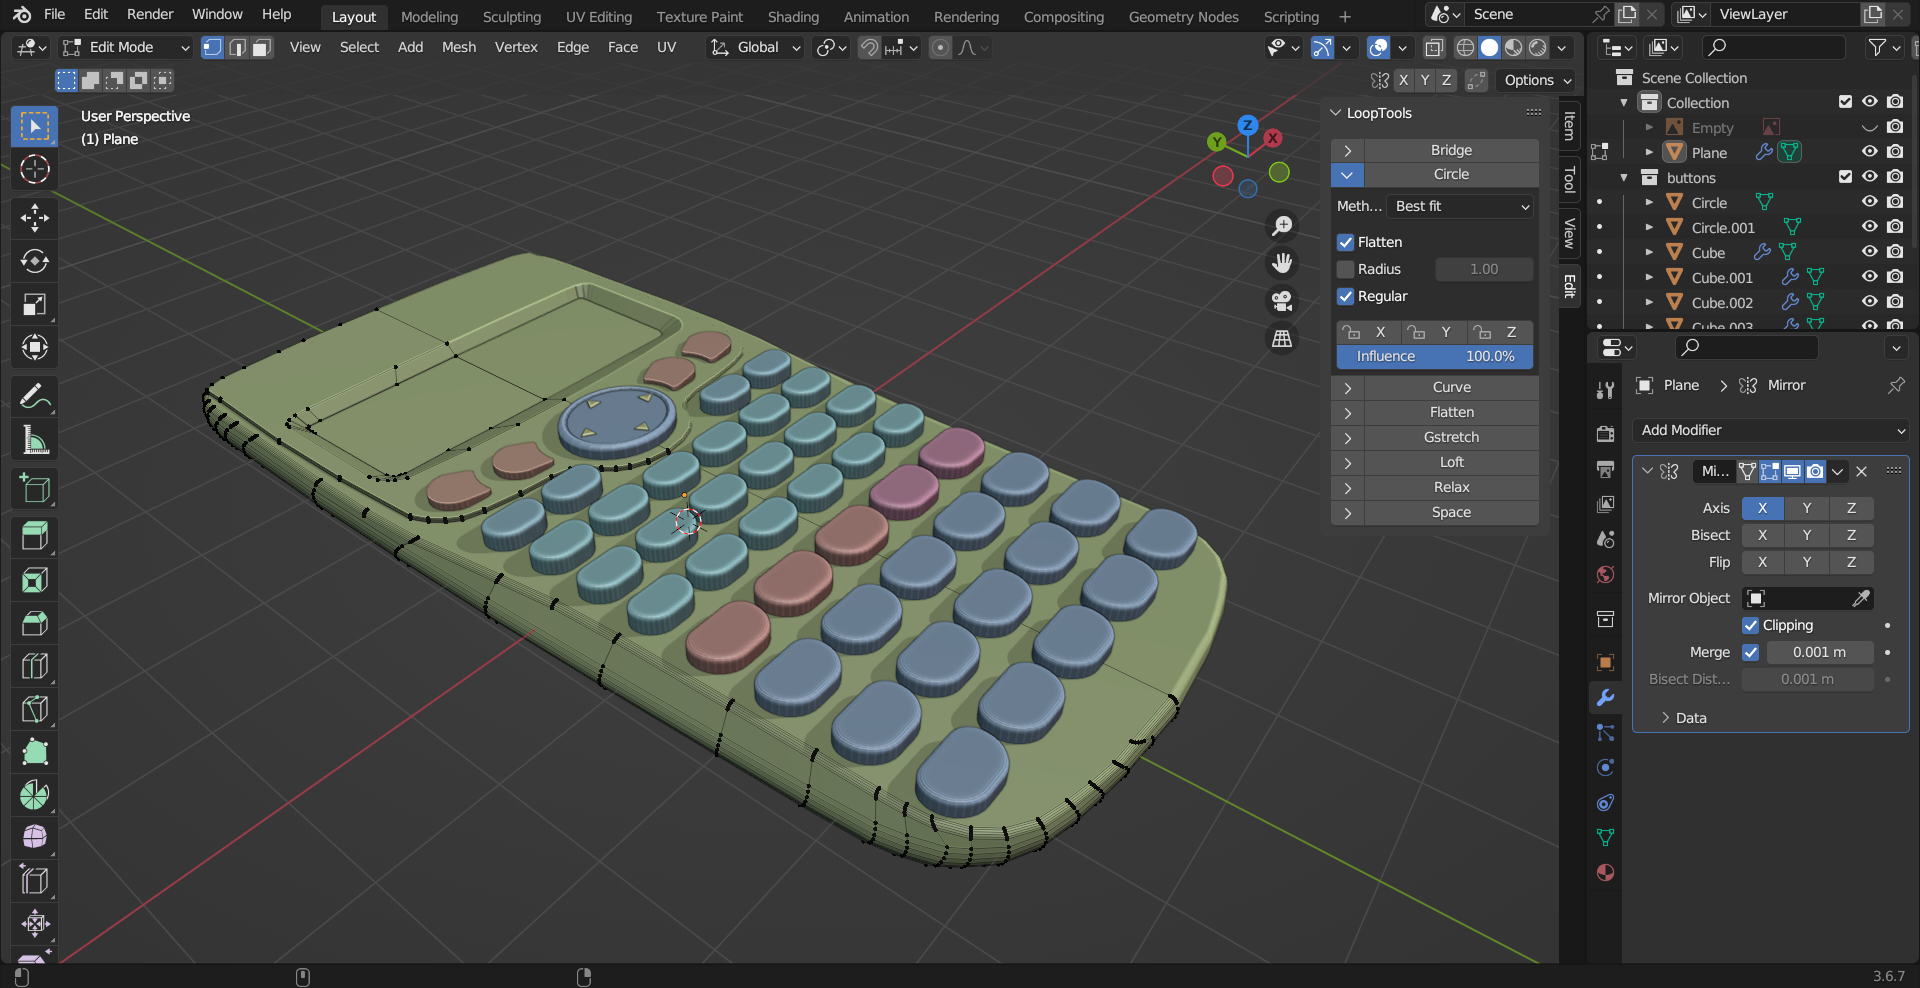
\includegraphics[width=1\textwidth]{images/calculatoreditmode.png}
    \caption{Edit Mode Ansicht auf das Calculator Objekt}
    \label{fig:calculatoreditmode}
\end{figure}
\end{comment}

\subsubsection{Wie funktioniert Blender im Allgemeinen?}

Die nachfolgende Beschreibung hebt die Schlüsselaspekte und die Funktionalität von Blender für unseren speziellen
Anwendungsbereich hervor.

\begin{itemize}
    \item \textbf{Benutzeroberfläche und Interaktion}\\
    Die Benutzeroberfläche von Blender ist komplex gestaltet, aber hoch anpassbar. Sie enthält 3D-Modelle,
    Ansichten, Fenster und Panels. Benutzer interagieren mit Objekten und Werkzeugen über Maus- und Tastaturbefehle,
    wobei erfahrene Nutzer Hotkeys oder Shortcuts verwenden können, um effizienter zu arbeiten.

    \item \textbf{3D-Modellierung}\\
    Blender ermöglicht die Erstellung von 3D-Modellen durch die Verwendung von Primitiven wie Würfeln, Kugeln,
    Flächen und Kurven. Diese können dann bearbeitet und modifiziert werden, um komplexe Formen zu erstellen.
    Modellierungswerkzeuge umfassen Extrusion, Verschiebung, Skalierung und Rotation.

    \item \textbf{Materialien und Texturen}\\
    Zur Erzeugung realistischer Oberflächen können Materialien erstellt und Texturen auf Objekte angewendet werden.
    Blender erlaubt die Feinanpassung von Materialeigenschaften wie Diffusreflexion, Glanz, Transparenz und Emission.

    \item \textbf{Gemeinschaft und Ressourcen}\\
    Blender verfügt über eine engagierte Benutzergemeinschaft, die umfassende Dokumentation, Tutorials und Foren
    bereitstellt. Diese Ressourcen erleichtern die Einarbeitung und die Lösung von Problemen.

\end{itemize}
Blender kommt in unserer Diplomarbeit in beiden Leveln zum Einsatz. Die Hauptanwendung des Programms findet im Level 2
statt, wo Blender für die digitale Modellierung wichtiger täglicher Gegenstände von Schülern genutzt wird. Das Ziel ist
es, am Ende eine umfangreiche Sammlung von Objekten zu haben, um den Benutzern eine vielfältige Auswahl zu bieten.